\documentclass[10pt]{article}
\usepackage[polish]{babel}
\usepackage[utf8]{inputenc}
\usepackage[T1]{fontenc}
\usepackage{amsmath}
\usepackage{amsfonts}
\usepackage{amssymb}
\usepackage[version=4]{mhchem}
\usepackage{stmaryrd}
\usepackage{graphicx}
\usepackage[export]{adjustbox}
\graphicspath{ {./images/} }
\usepackage{hyperref}
\hypersetup{colorlinks=true, linkcolor=blue, filecolor=magenta, urlcolor=cyan,}
\urlstyle{same}

\title{GIMNAZJUM }

\author{}
\date{}


\begin{document}
\maketitle
\begin{enumerate}
  \item Dany jest 17-kąt foremny. Wybrano jego 10 wierzchołków. Wykaż, że wśród wybranych punktów są cztery będące wierzchołkami trapezu.
  \item Rozwiąż układ równań:
\end{enumerate}

\[
\left\{\begin{array}{l}
x^{2}+24=9 y+\frac{x+z}{2} \\
y^{2}+25=9 z+\frac{x+y}{2} \\
z^{2}+26=9 x+\frac{y+z}{2}
\end{array}\right.
\]

\begin{enumerate}
  \setcounter{enumi}{2}
  \item Dane są trzy parami styczne zewnętrznie okręgi o promieniu 1. Wyznacz pole trójkąta, którego boki są odcinkami stycznych.\\
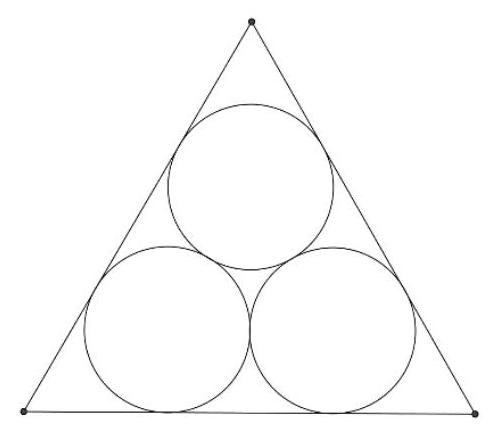
\includegraphics[max width=\textwidth, center]{2024_11_21_e501b0bc4e839ef815dfg-1}
\end{enumerate}

\section*{LICEUM}
\begin{enumerate}
  \item Dane są punkty \(A=(-5,0), B=(-3,-4), C=(3,4), M=(7,1)\). \(Z\) punktu \(M\) poprowadzono styczne \(k\) i \(l\) do okręgu opisanego na trójkącie \(A B C\). Oblicz pole trójkąta \(K L M\), gdzie \(K\) i \(L\) są punktami styczności prostych \(k\) i \(l z\) tym okręgiem.
  \item Oblicz sumę \(n\) początkowych wyrazów ciągu \(\left(a_{n}\right), \mathrm{w}\) którym\\
\(a_{1}=3, a_{2}=33, a_{3}=333, a_{4}=3333, \ldots\)
  \item W półokrąg o promieniu \(R\) wpisano trapez, w którym ramię jest nachylone pod kątem \(\alpha\) do podstawy będącej średnicą okręgu. Oblicz pole trapezu.
\end{enumerate}

Rozwiazzania należy oddać do piątku 6 listopada do godziny 10.35 koordynatorowi konkursu panu Jarostawowi Szczepaniakowi lub swojemu nauczycielowi matematyki lub przestać na adres \href{mailto:jareksz@interia.pl}{jareksz@interia.pl} do piątku 6 listopada do pótnocy.


\end{document}